\subsection{Scenario-Based Design}
Scenarios are a foundation for the design of interactive systems. Scenario ``engineering'' involves requirements work, prototyping, envisionment, evaluation, conceptual design and physical design.

\begin{figure}[h!]
	\centering
	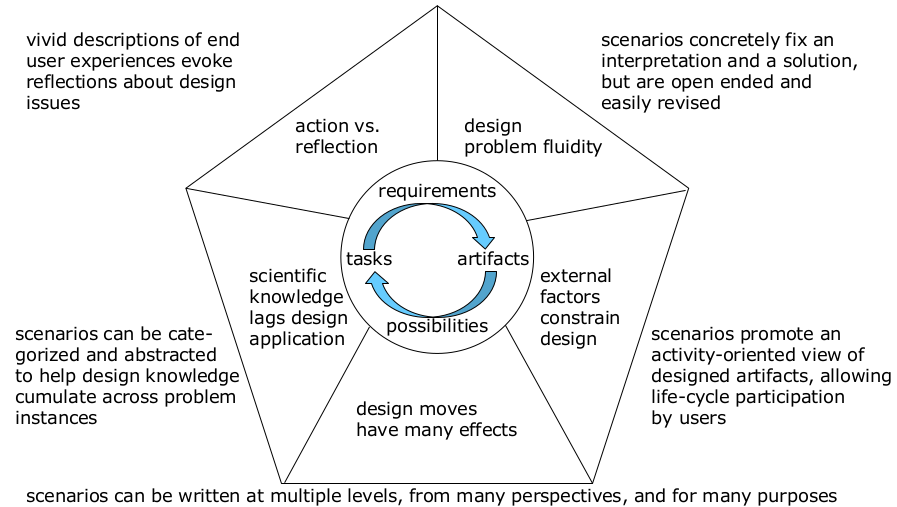
\includegraphics[width=.8\textwidth]{img/ch06_scene.png}
	\caption{Challenges and Approaches in Scenario-based Design}
	\label{scen}
\end{figure}
\textbf{Design rationale}: making the reasons for design decisions explicit. Methods for capturing and representing design rationale:\\
IBIS – issues, positions, arguments and relations
QOC – questions, options and criteria (graphical links)\\

\begin{figure}[h!]
	\centering
	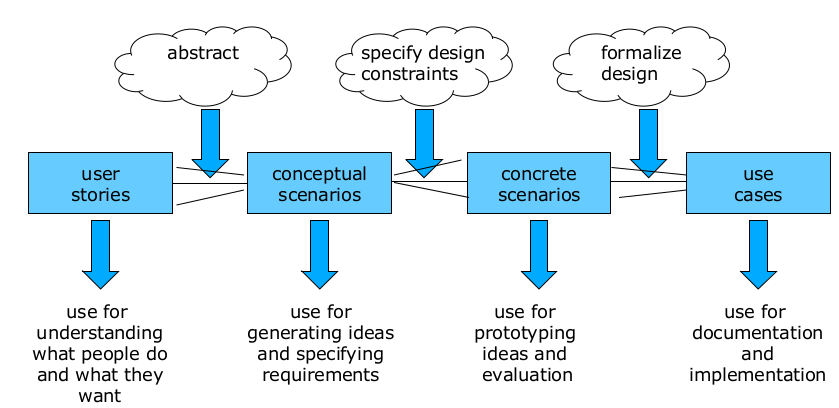
\includegraphics[width=.8\textwidth]{img/ch06_scene1.png}
	\caption{Scenarios in the Design Process}
	\label{scen1}
\end{figure}

\textbf{User Stories}: reveal ideas, anecdotes, knowledge of people, real-world experiences, activities and context. They are used to identify the problem, the stakeholders and their constraints.\\

\textbf{Conceptual Scenarios}: more abstract than user stories, derived by combining several user stories. The are used for generation of ideas and understanding requirements but do not include technology and do not specify how functions are provided.\\

\textbf{Concrete Scenarios}: derived and generated by conceptual scenarios; each conceptual scenario may generate many concrete scenarios. They suggest a particular user interface design and helü allocating functions between devices and people. They form a good start for prototyping and evaluation. \\

\textbf{Use Cases}: may result from many concrete scenarios and describe the interaction between devices and people. They abstract from concrete scenarios. Each use case covers many slight variations. Allocation of tasks and functions is needed for a use case. The sum of all use cases specifies the system design. Use cases may consist of diagrams, pseudo code, etc.

\begin{figure}[h!]
	\centering
	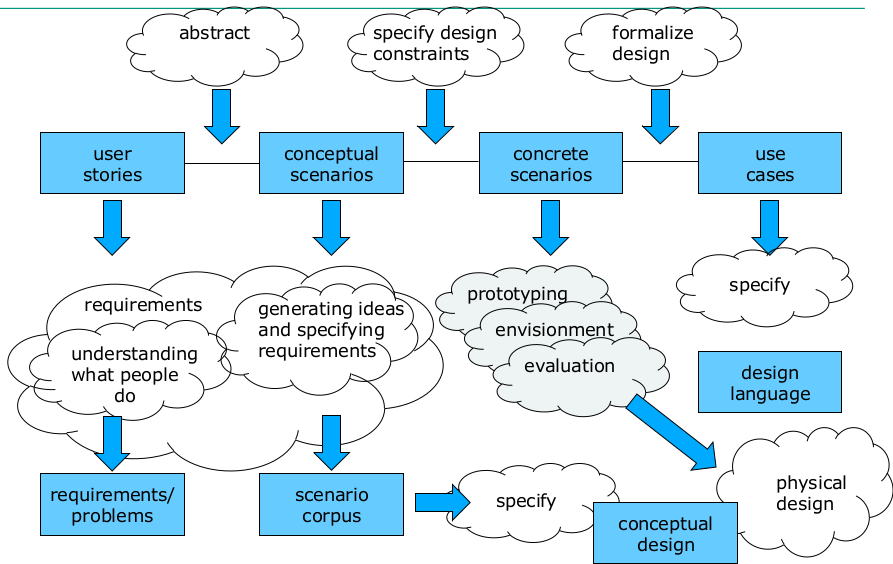
\includegraphics[width=.8\textwidth]{img/ch06_scene2.png}
	\caption{Overall Scenario-Based Design}
	\label{scen2}
\end{figure}

\textbf{Requirements and Problems}: By analysis and abstractions, difficulties become visible. In general these steps allow designers to collect experience in the formative process, in which requirements (desirable qualities of the system) can be derived. Prioritization is necessary since not all properties will be realizable.\\

\textbf{Scenario Corpus}: One wants to create a representative set of scenarios that cover a wide range of user stories. Some may be more specific, some may be more general but one takes a high-level, abstract view of the most activities in order to uncover the dimensions of the systems and the involved domains. If you don't do this, the outcome is most likely determined by technical features rather than by user requirements.\\

\textbf{Conceptual Model/Design}: An object or data model includes scenario and analysis of scenarios and describes the main objects, attributes and relationships among them. It ensures an accurate mental model of the interactive system. Here an analysis of cognitive processes, e.g. cognitive load, conceptualization is required. For example the desktop is a metaphor (mental model) for your desk.\\ 

\textbf{Design Language}: A standard set of patterns for interaction. General Design Language Concepts may be in place before concrete design application (e.g. Company Design Guidelines). Interaction patterns include physical attributes, conceptual actions and objects, key elements of design as well as principles and rules. Common language reduces the number of elements for the involved designers.

\subsection{Requirements}
Requirement analysis means understanding what people do, what people might want to do, problems with existing systems, and how people do what they do. The goal is to create ``better'' interactive systems for people. According to Robertson and Robertson (1999) a requirement is ``... something the product must do or a quality that the product must have''. Requirement work is the transformation of observation and information . It requires iterations on analysis, design, and evaluation and results in a requirements specification (formal and precise documentation of the requirements). User stories are a good start for user requirement analysis. The design process helps identifying requirements. Requirement Analysis work is very similar to software engineering! Two types:
\begin{itemize}
\item functional requirements: specify what the system must do; e.g. phone function button must be accessible while connected to the internet
\item non-functional requirements: specify what qualities the system must have, concerned with how the functionality operates; e.g. an elderly person must be able to use the phone
\end{itemize} 
For both requirement types, the technology is not yet specified, i.e. there is no specification of the implementation how-to, only usage how-to!\\
Not all requirements have equal impact on the interactive systems. Since resources are limited one needs prioritization and good balance.\\
MoSoCoW rules for prioritizing requirements:
\begin{itemize}
\item \textbf{m}ust have: fundamental requirements without which the system will be unworkable and useless, effectively the minimum usable set
\item \textbf{s}hould have: would be essential if more time were available, but the system will be useful and usable without them
\item \textbf{c}ould have: of lesser importance, therefore can more easily left out of the current development
\item \textbf{w}ant to have: will not have this time round, can wait till a later development
\end{itemize}
One may use a requirement template for functional and non-functional requirements, for project (time, man power) and design (technology) constaints:

\begin{figure}[h!]
	\centering
	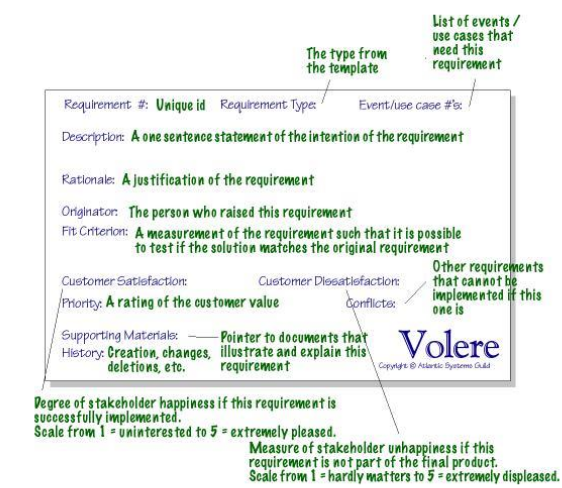
\includegraphics[width=.8\textwidth]{img/ch06_req.png}
	\caption{Using a requirement template.}
	\label{req}
\end{figure}
One can define four requirements activities, which all have the same goal:
\begin{itemize}
\item requirements gathering, which suggests requirements are lying around waiting to be picked up / explored with little interaction between designer and user. Cons: unstructured
\item requirements generation, which suggests a more creative designer activity, but tends to de-emphasize links to users' current practice.
Pros: creative. Cons: not user centered
\item requirements elicitation, suggests some user-designer interaction. Pros: user-designer collaboration. Cons: May stuck to user's creativity
\item requirements engineering, used in software engineering, suggests a very formal approach. Pros: goal oriented. Cons: formalizing to early, kills creativity
\end{itemize}
There are numerous techniques for requirements elicitation/gathering: interviews, observations, documentation (e.g. video-taping), focus groups, workshops.. (c.f. Chapter Observation). No matter which techniques are used: requirements elicitation is a user-centered activity!\\
Interviews, questionnaires and observation will identify artifacts used during the task. Most tasks require artifacts to complete. Artifacts provide additional insight in the task. Examples are documents, forms, printouts, tools..

\subsection{Envisionment}
Envisionment is concerned with making ideas visible by externalizing thoughts. The goal is to represent design work to the designers and stakeholders using stories and scenarios, presentations, sketches, formal models, software and hardware prototypes, cardboard models, mockups, ...This is fundamental to user-centered design and enables designers to see things from other people's perspective and to communicate ideas to people. It serves for generation, communication and evaluation of ideas but not all representations are suitable for all setups!\\
Exploring design concepts:
\begin{itemize}
\item how do you do it? $\rightarrow$ how do we affect the world (manipulate, sit, etc.); examples: handles (continuous) vs. buttons (discrete)
\item how do you feel? $\rightarrow$ how does the user make sense of the world, sensory qualities that shape media; satisfaction, affect, enjoyment, engagement, involvement
\begin{itemize}
\item hot media (photo): exact, authoritative, extend a single sense
\item cool media (cartoon): fuzzy and incomplete
\end{itemize}
\item how do you know? $\rightarrow$ how do people learn and plan; how designers want users to think; example: paths vs. maps (step by step vs. understanding alternatives)
\end{itemize}
\textbf{Sketches}: sketching (quickly drawing ideas and thoughts) is an important ability of a designer and used for exploration and discussion. Many ideas have been sketched out on ``the back of an envelope'' or on a napkin. Shneiderman's principle for sketches: ``overview first, zoom and filter, then details on demand'' (similar for Web-Site design!)\\
\textbf{Snapshots}: show key moments in an interaction, often refined sketches; exploring the impact of a certain style or design snapshots by sketches, storyboards or using software (e.g. Macromedia Flash, HTML, ...)\\
\textbf{Storyboards}: Technique from film making. Cartoon-like structure presenting key moments from the interactive experience: This allows people to get an idea of the flow and is an economical way to present design (6-8 scenes on one paper). There are three main types of storyboards:
\begin{itemize}
\item traditional storyboarding: as in filmmaking; scenes with notes to overcome static nature of scenes on paper; annotations of interactive behavior; good for non-multimedia user interfaces
\item scored storyboards: good for applications with motion graphics; annotation and notes about the type, colors, images, sounds
\item text-only storyboards: used for applications with complex sequences; specifies what images appear, what text comes with them, and any additional media, ...
\end{itemize}
\textbf{Mood boards} gather visual stimuli that capture something about the feeling of the design. They are widely used in advertising and interior design and may feature photographs, colors, textures, shapes, headlines from newspapers or magazines, quotations from people, pieces of fabric, ...\\
\textbf{Cultural probes} (Gaver, 1999) allow involvement and creativity and are about getting to know your target group. You prepare a set of common items (introduction how to use and what to do with the material, e.g. booklet, maps, postcards, ...; suitable prototypes). You give the items to the participants and let them use it over a certain period of time. Not all items might be used as envisioned!\\
\textbf{Navigation Maps}: Navigation is a key feature for many (complex) systems. Find out, how the user moves through the site or applications focussing on how users will experience the site. This is used to uncover functional complexity of the system and to reduce recognized complexity by better grouping navigational elements. Each page in the site or location in the application is represented with a box or heading; each page should ``flow'' from there. Navigation maps can be redrawn many times during the project lifecycle – poor navigation is a main reason to turn off customers e.g. from a website.\\
\textbf{Scenarios in Envisionment}: Scenarios, in their most concrete form, can be used to envision or evaluate specific interactions.\\
Concrete scenario $\rightarrow$  prototyping $\rightarrow$  envisonment scenarios in the figure\\
The aim is to complement scenarios with some of the more visual envisioning techniques. Scenarios in envisionment should include real data and materials to allow direct involvement and you should think hard about underlying assumptions. You should also include good characterizations and develop a good number of personas. This allows ``talking'' about the characters. Also provide rich contextual background grounding in real life forces to think about practicality and acceptability. It is impossible to write scenarios for all variations and users, but the produced scenarios should cover interactions which are typical for a number of similar use situations, important design issues which are particularly important for the focus of the project, areas where requirements are unclear, and any aspects which are safety-critical. Scenarios should be structured (e.g. title, activities, rationale). When writing, thinking about or using scenarios, issues will arise about the design space. Only when people ``see'' a concrete representation, they are able to comment meaningfully. This is achieved by e.g. notes on the storyboards, or end notes to the scenario. Often, requirements will have to be changed. You should list positive and negative features for a concrete design (capturing rationale). Scenarios are effective to bring open issues to the surface.\\
\textbf{An Outline Envisionment Process}:
\begin{itemize}
\item[1)] Review the requirements and conceptual scenarios
\item[2a)] Develop representations of the design ideas. These should include: concrete scenarios, storyboards, snapshots and sketches, ..
\item[2b)] Alternatives: If your product is a new one, experiment with different metaphors and design concepts through your representations
\item[2c)] Users: Your intended users should be involved in exploring design ideas throughout wherever possible
\item[3)] Decisions: Resources permitting, explore and document detailed design decisions using a method such as Questions, Options, Criteria (QOC)
\item[4)] Reconsider requirements in the light of the developing design, and carry out supplementary analysis where gaps in your background information have been uncovered.
\end{itemize}
\subsection{Prototyping}
Prototyping is an effective way for communicating ideas and design and complements/precedes techniques for envisionment. It is important to select the appropriate techniques. There are different levels of prototypes. Prototyping allows for participatory designs. Prototypes are a concrete but partial representation or implementation of a system. So far, screen sketches where discussed. These are, however, not interactive. Prototyping is a participatory design activity.
You could either have deep/vertical prototypes or shallow/horizontal prototypes.\\
\textbf{High Fidelity Prototypes} are  similar in look and feel to the anticipated final system. They are produced in the software that will be used for implementation or using a ``simulation'' package (e.g. using graphical toolkit: Flash, etc.) and useful for a detailed evaluation of the main design elements (content, visuals, interactivity, functionality and media). Hi-fi prototypes are also used in crucial stages of the project, e.g. client acceptance tests. They are used when the ideas, requirements and features of the system become stable. However, people might believe that the final system will exactly like the prototype! Also, a hi-fi prototype suggests that the system can be implemented/made to work! Hi-fi prototypes are costly!\\
\textbf{Low Fidelity Prototypes} are more focused on the underlying ideas, such as content, form and structure, key functionality requirements and navigational structure. They are designed to be produced quickly and thrown away after use and capture very early design thinking and should aid, not hinder, the process of generating and evaluating many possible design solutions. They often come in the form of paper prototypes (printout, paper, pen, post-its), series of screen shots. Paper prototypes are often an ideal means of prototyping interactive, screen-based systems!
Practical issues with designing paper prototypes are:
\begin{itemize}
\item robustness: can be handled by many ``users'' without breaking -- unlike a ``soldered together piece of electronics''...
\item scope: focus on broad issues and key elements; too detailed is hard to understand
\item instructions: trade-off between adding enough detail to allow the user alone to explore and between adding too much detail (so the designer needs to walk the user through)
\item flexibility: have adjustable parts (e.g. lay over other printouts e.g. on a menu, text box, ...) for visualizing interactive parts
\end{itemize}
Lo-fi prototypes usually do not ``work'' -- the designer is needed to play the computer (Wizard of Oz). Videotaping the ``interaction'' if there is much feedback. User guidance to help people access the prototype, e.g. ``setting the scene'' for a new UI for a web shop: ``You are interested in buying the shirt shown on this screen but want to know more about the material – show me what you would do now.'' Alternatively, if the system is too fragile to be exposed to users, the designers might act under the user's guidance. Much cheaper than Hi-fi, much cheaper than re-design!\\
\textbf{Trade Offs}: LoFi or HiFi Prototypes? What and how to prototype? $\rightarrow$ think in terms of PACT. Who is the prototype aimed at? What is the designer trying to achieve with the prototype? What stage of the project are things at and what is the context for use of the prototype? What technologies are appropriate?\\
According to Rosson and Carrol (2002) High-quality graphics and animation can be used to create convincing and exciting prototypes but may also lead to premature commitment to some design decision? Detailed special-purpose prototypes help to answer specific questions about a design, but building a meaningful prototype for each issue is expensive. Realistic prototypes increase the validity of user test data, but may postpone testing, or require construction of throw-away prototypes. Iterative refinement of an implementation enables continual testing and feedback, but may discourage consideration of radical transformations. Test users just get tired/used to the system.\\
Prototyping is necessary during the whole design process, but seldom done. Prototyping is much cheaper / leads to faster solution than re-implementation or project failure. ``requirements animation'': illustrating requirements by use of prototypes. Rapid prototyping for exploring the design space. Throw-away prototypes as part of the rapid prototyping activity to test/verify assumptions, but: ``You will throw away your first few designs, so you might as well plan to throw them away in the first place''.\\
\textbf{Prototype Tools}: 
\begin{itemize}
\item for requirements animation might include: PowerPoint, paper (and paper overlays), Visual Basic
\item for throw away/rapid prototyping: Adobe Flash, Web Tools
\item for incremental/evolutionary prototyping: development environment, object-oriented languages
\item for physical user interfaces: clay, wood, ..., 3D printers
\end{itemize}